% !TEX root = Theo_III.tex

\usepackage{tikz}
\usetikzlibrary{arrows.meta,positioning,decorations.markings,intersections,calc,decorations.pathreplacing,external}
%\tikzexternalize[prefix=figures/] % activate

\tikzset{
    object color/.style={blue!40!black!80!white},
    object style/.style={object color,thick},
    legreen/.style={green!50!black},
    lorange/.style={red!60!yellow!70!black!90!white},
    polarisation color/.style={purple},
    charge color/.style={blue!50!white!70!black},
    red laser/.style={red!70!black},
    moving system color/.style={blue!60!black!70!white},
    coordsystem/.style={very thin, color=#1!50},
    invisible point/.style={circle,inner sep=0pt,outer sep=0pt,minimum size=0pt},
    point/.style={invisible point,fill=black,minimum size=4pt},
    arr/.style={->,>={Stealth},thin},
    rarr/.style={<-,>={Stealth},thin},
    midarrow/.style={postaction=decorate,decoration={markings, mark=at position #1 with {\arrow{Stealth}}} },
    midarrow/.default=.5,
    rmidarrow/.style={postaction=decorate,decoration={markings, mark=at position #1 with {\arrowreversed{Stealth}}} },
    rmidarrow/.default=.5,
    distance marker/.style={|<->|,>={Stealth}},
}
\tikzstyle{every node}=[font=\footnotesize]


\newcommand{\tfigTitel}{
    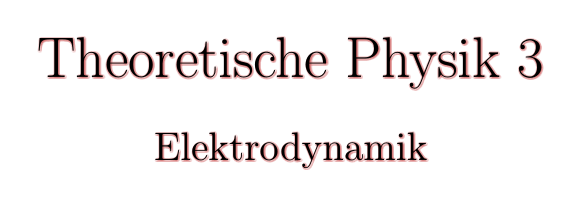
\begin{tikzpicture}
        \pgfmathsetmacro{\shadowangle}{132}
        \newlength{\shadowdistance}
        \pgfmathsetlength{\shadowdistance}{0.1ex}
        \pgfmathsetmacro{\shadowopacity}{1}
        \pgfmathsetmacro{\shadowspread}{0.003}
        \pgfmathsetmacro{\shadowsize}{5}
        \pgfmathtruncatemacro{\totshadow}{100}
        \path[red laser,opacity={\shadowopacity/\totshadow},shift={({132-180}:\shadowdistance)},scale={1+\shadowsize}] 
        foreach \nshadow [evaluate=\nshadow as \angshadow using \nshadow/\totshadow*360] in {1,...,\totshadow}{
            node[align=center] at (\angshadow:\shadowspread) {\huge Theoretische Physik 3\\ \\ \\
            \Large Elektrodynamik}
            };
        \node[align=center] at (0,0) {\huge Theoretische Physik 3\\ \\ \\ \Large Elektrodynamik};
    \end{tikzpicture}
}

\newcommand{\tfigVolumeWithNormal}{
    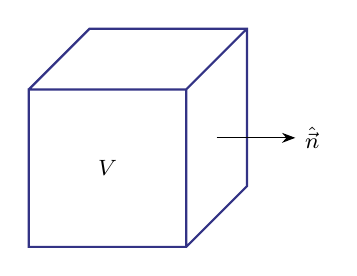
\begin{tikzpicture}[scale=2]
        \draw[object style] (0,1,1) -- (0,1,0) -- (1,1,0) -- (1,0,0)
        -- (1,0,1) -- (0,0,1) --(0,1,1) -- (1,1,1) 
        -- (1,0,1) --  (1,1,1) -- (1,1,0);
        % \node at (.5,.5,1) {$\vec a(\vec r)$};
        \node at (.5,.5,1) {$V$};
        \draw[arr] (1,.5,.5) -- +(0.5,0,0) node[right] {$\hat{\vec n}$};
    \end{tikzpicture}
}

\newcommand{\tfigAreaWithCurveAndNormal}{
    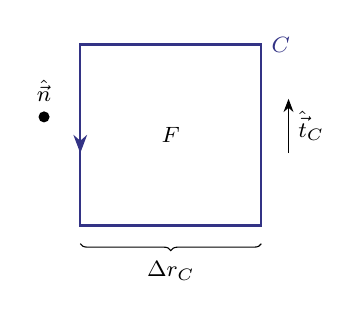
\begin{tikzpicture}[scale=2.3]
        \draw[object style,rmidarrow=.1] (0,0) rectangle (1,1) node[below,right] {$C$};
        \node at (.5,.5) {$F$};
        \node[point, label={$\hat{\vec n}$}] at (-.2,.6) {};
        \draw[decorate, decoration = {brace, mirror}]  (0,-.1) -- +(1,0) node[midway, below,yshift=-3pt] {$\Delta r_C$};
        \draw[arr] (1.15, .4) -- +(0,.3) node[midway, right] {$\hat{\vec t}_C$};
    \end{tikzpicture}
}

\newcommand{\tfigLinienintegral}{
    \begin{tikzpicture}[scale=2, clr/.style={lorange}]
        \coordinate (A) at (0,0);
        \coordinate (NC) at (0,.2);
        \coordinate (B) at (1.3,2);
        \coordinate (FC) at (.5,.1);
        \coordinate (C2) at (1.5,1);
        \coordinate (R) at (0.65,1);
        
        \node[point, label=right:{$\vec r_0$}] at (A) {};
        \node[point, label=right:{$\vec r_1$}] at (B) {};
        
        \draw[object style] (A) .. controls ($(A)+(NC)$) and ($(R)-(FC)$) .. (R) .. controls  ($(R)+(FC)$) and ($(B)-(NC)$) .. (B)
          node[very near end, left] {$C$};
        
        \node[point,clr,label={below,clr}:{$\vec r$}] at (R) {};
        \draw[arr,clr] (R) -- ($(R)+(FC)$) node[below] {$\diff \vec r$};
        \draw[arr, legreen] (-.1,.2) -- (-.01,.5) node[midway, left] {$s$};
    \end{tikzpicture}
}

\newcommand{\tfigHalbkugel}{
    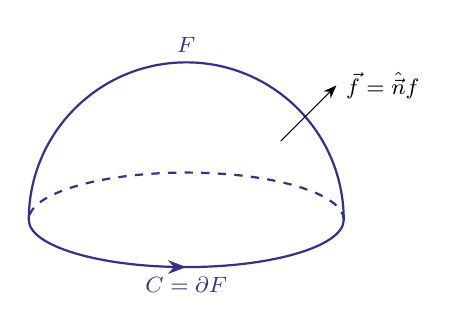
\begin{tikzpicture}[scale=2]
        \coordinate (A) at (0,0);
        \draw[object style] (0,0) arc (0:180:1) node[midway, above] {$F$};
        \draw[object style,dashed] (0,0) arc (0:180:1 and .3);
        \draw[object style,rmidarrow] (0,0) arc (0:-180:1 and .3) node[midway, below] {$C=\partial F$};
        
        \draw[arr] (-.4,.5) -- +(45:.5) node[right] {$\diff \vec f=\hat{\vec n}\diff f$};
    \end{tikzpicture}
}

\newcommand{\tfigCoulombPointCharges}{
    % Forces on to charges
    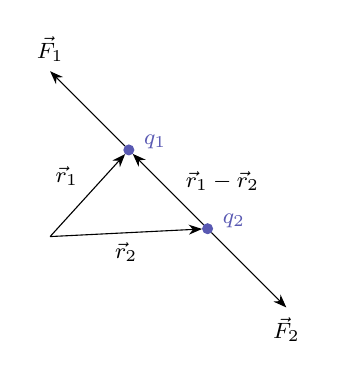
\begin{tikzpicture}[scale=1]
        \coordinate (O) at (0.0,0.0);
        \coordinate (Q1) at (1.0,1.1);
        \coordinate (Q2) at (2.0,.1);
        \coordinate (F1) at ($(Q1)+(Q1)-(Q2)$);
        \coordinate (F2) at ($(Q2)+(Q2)-(Q1)$);
        
        \node[point, charge color] (Q1 node) at (Q1) 
            [label={east, yshift=1mm, charge color}:$q_1$] {} 
            edge[arr] node[at end, above] {$\vec F_1$} (F1);
        \node[point, charge color] (Q2 node) at (Q2) 
            [label={east, yshift=1mm, charge color}:$q_2$] {} 
            edge[arr] node[at end, below] {$\vec F_2$} (F2)
            edge[arr] node[midway, right, yshift=1mm, xshift=1mm] {$\vec r_1-\vec r_2$} (Q1 node);
        \node[invisible point] at (O) {} 
        edge[arr] node[midway, below] {$\vec r_2$} (Q2 node)
        edge[arr] node[midway, anchor=south east] {$\vec r_1$} (Q1 node);
    \end{tikzpicture}
}

% äquipotentiallinien und elektrische feld Linien zweier ungleichnamiger ladungen
\newcommand{\tfigDipoleFieldPotential}{
    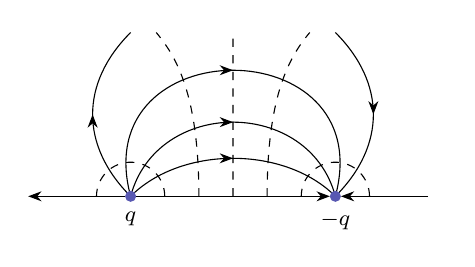
\begin{tikzpicture}[scale=1.3]
        \coordinate (Q1) at (-1,0);
        \coordinate (Q2) at (1,0);
        \coordinate (A1) at (-2,0);
        \coordinate (A2) at (2,0);
        \coordinate (T) at (0,1.6);
        \draw[midarrow] (Q1) .. controls +(45:.7) and +(135:.7) .. (Q2);
        \draw[midarrow] (Q1) .. controls +(75:1)  and +(105:1)  .. (Q2);
        \draw[midarrow] (Q1) .. controls +(105:1.7) and +(75:1.7) .. (Q2);
        \draw[midarrow] (Q1) .. controls +(135:.7) and +(-135:.7) .. ($(Q1)+(T)$);
        \draw[rmidarrow] (Q2) .. controls +(45:.7) and +(-45:.7) .. ($(Q2)+(T)$);
        
        \draw[dashed] 
            let \p1=(Q1),\p2=(Q2) in
            (0,0) -- (T)
            (\x1/3,0) .. controls +(90:1) and +(-50:.3) .. ($(T)+{3/4}*(Q1)$)
            (\x2/3,0) .. controls +(90:1) and +(-130:.3) .. ($(T)+{3/4}*(Q2)$)
            (\x1-\x1/3,0) arc(0:180:1/3)
            (\x2+\x2/3,0) arc(0:180:1/3);
        
        \node[point, charge color] (Q2 node) at (Q2) 
            [label=south:$-q$] {} ;
        \node at (A2) {} 
            edge[arr] node {} (Q2 node);
        \node[point, charge color] (Q1 node) at (Q1) 
            [label=south:$q$] {} 
            edge[arr] node {} (A1)
            edge[arr] (Q2 node);
    \end{tikzpicture}
}

\newcommand{\tfigEfieldAndPotLinesAndChargeDensitityHomoChargedSphere}{
    % Field and equipotential lines of a charged sphere
    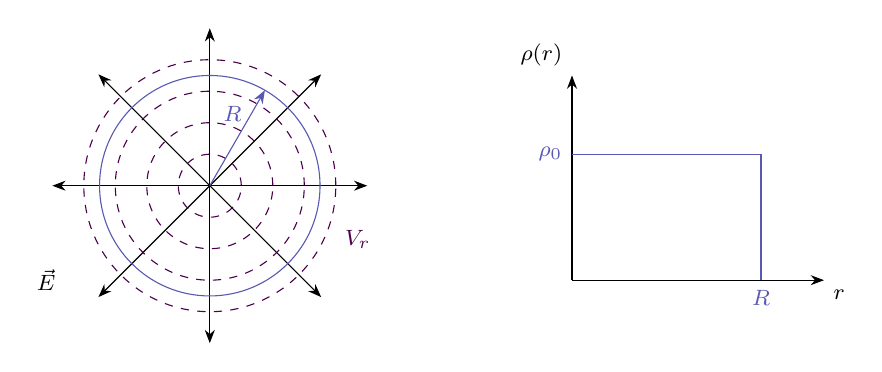
\begin{tikzpicture}[
        scale=2,
        potential color/.style={violet!60!black}
    ]
    \coordinate (O) at (0.0,0.0);

    \foreach \angle in {0,45,...,325}
        \draw[arr] (O) -- (\angle:1);
    \foreach \radius in {0,0.2,...,0.8}
        \draw[dashed,potential color] (O) circle [radius=\radius];
        
    \node[potential color] at (-20:1) {$V_r$};
    \node at (-150:1.2) {$\vec E$};

    \draw[charge color] (O) circle [radius=.7];
    \draw[arr, charge color] (O) -- (60:0.7) node[near end, left] {$R$};

    \begin{scope}[shift={(2.3,-.6)}]
        \coordinate (A) at (1.2, 0.8);
        
        \draw[arr] (0,0) -- (0, 1.3) 
            node[at end, anchor=south east] {$\rho(r)$};
        \draw[arr] (0,0) -- (1.6, 0) 
            node[at end, anchor=north west] {$r$};
        \draw[charge color] let \p1 = (A) in
            (0, \y1) -- (A) 
            node[at start, left] {$\rho_0$}
            -- (\x1, 0)
            node[charge color, below] {$R$};
    \end{scope}
    \end{tikzpicture}
}
\newcommand{\tfigEfieldAndPotentialHomoChargedSphere}{
    % field and potential function for sphere
    \begin{tikzpicture}[scale=3]
        \coordinate (A) at (0.8, 0.8);
        
        % electric field
        \draw[arr] (0,0) -- +(0, 1.1) 
            node[at end, anchor=south east] {$E(r)$};
        \draw[arr] (0,0) -- +(1.8, 0) 
            node[at end, anchor=north west] {$r$};
            
        \draw[charge color,yscale=.2] 
            let \n1={0.5},\n2={1.7} in
            plot[domain=0:\n1] (\x,\x/\n1^3) 
            node[above left] at (\n1/2,\n1/2/\n1^3) {$\propto r$} 
            plot[domain=\n1:\n2] (\x,1/\x^2) 
            let \n4={.5*\n2-.5*\n1+\n1} in % x value of middle point of second graph 
            node[above] at (\n4,1/\n4^2) {$\displaystyle\propto\frac{1}{r^2}$};
        \draw[dashed, very thin] (0.5,.8) -- +(0,-.8) 
            node[below] {$R$};
            
        % potential
        \begin{scope}[shift={(2.5,0)}]
            \draw[arr] (0,0) -- +(0, 1.1) 
                node[at end, anchor=south east] {$\phi(r)$};
            \draw[arr] (0,0) -- +(1.8, 0) 
                node[at end, anchor=north west] {$r$};
            \draw[charge color,yscale=.3] 
                let \n1={0.5},\n2={1.7} in 
                plot[domain=0:\n1] (\x,3/\n1/2 -\x^2/\n1^3/2)
                node[right, xshift=-25,yshift=25] {$\displaystyle\propto \frac3{2R}-\frac{r^2}{2R^3}$}
                plot[domain=\n1:\n2] (\x,1/\x)
                let \n4={.5*\n2-.5*\n1+\n1} in % x value of middle point of second graph 
                node[above] at (\n4,1/\n4) {$\displaystyle\propto\frac{1}{r}$};
                
            \draw[dashed, very thin] (0.5,1/1.7) -- +(0,-1/1.7) 
                node[below] {$R$};
        \end{scope}
    \end{tikzpicture}
}

\newcommand{\tfigThreeConductors}{
    % Anordnung von elektrischen Leitern Li mit Ladungen Qi und Potentialen φi.
    \begin{tikzpicture}[clr/.style={legreen},scale=1.2]
        \draw[rotate=45] 
            (0,0) ellipse [x radius=1.2, y radius=.5] 
            node {$L_1$} node[charge color] at +(-.9,0) {$Q_1$}
            node[clr] at +(.2,.8) {$\phi_1$} ;
        \draw[rotate=0] 
            (2,-2) ellipse [x radius=.5, y radius=.55] 
            node {$L_2$} node[charge color] at +(-.5,-.6) {$Q_2$}
            node[clr] at +(.2,.8) {$\phi_2$};
        \draw[rotate=3] 
            (4,0) ellipse [x radius=.8, y radius=.4] 
            node {$L_3$} node[charge color] at +(-.5,-.6) {$Q_3$}
            node[clr] at +(.3,.6) {$\phi_3$};
        \node at (5,-1.4) {$\ldots$};
    \end{tikzpicture}
}

\newcommand{\tfigSpecialCapacitors}{

% capacitors
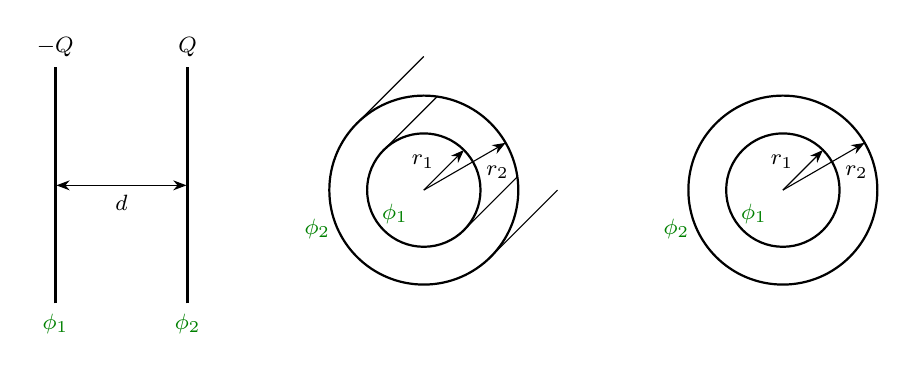
\begin{tikzpicture}[scale=1.2]
    \begin{scope}
        \coordinate (A0) at (-.7,0);
        \coordinate (A1) at (-.7,2.5);
        \coordinate (B0) at (.7,0);
        \coordinate (B1) at (.7,2.5);
        \draw[very thick] (A0) -- (A1) 
        node[at start,below,legreen] {$\phi_1$}
        node[at end,above] {$-Q$};
        \draw[very thick] (B0) -- (B1) 
        node[at start,below,legreen] {$\phi_2$}
        node[at end,above] {$Q$};
        
        \draw[distance marker] ($(A0)!.5!(A1)$) -- ($(B0)!.5!(B1)$) node[midway,below] {$d$};
    \end{scope}
    
    \begin{scope}[shift={(3.2cm,1.2cm)}]
        \coordinate (O) at (0,0);
        \draw[thick] (O) circle[radius=.6];
        \draw[thick] (O) circle[radius=1];
        
        \draw[arr] (O) -- (30:1) node[pos=.9, below,yshift=-3] {$r_2$};
        \draw[arr] (O) -- (45:.6) node[midway, above, left,yshift=3] {$r_1$};
        \node[legreen] at (-160:1.2) {$\phi_2$};
        \node[legreen] at (-140:.4) {$\phi_1$};
        
        \draw (135:1) -- +(45:1) (-45:1) -- +(45:1);
        \begin{scope}
            \clip (O) circle[radius=1];
            \draw (135:.6) -- +(45:1) (-45:.6) -- +(45:1);
        \end{scope}
    \end{scope}
    
    \begin{scope}[shift={(7cm,1.2cm)}]
        \coordinate (O) at (0,0);
        \draw[thick] (O) circle[radius=.6];
        \draw[thick] (O) circle[radius=1];
        
        \draw[arr] (O) -- (30:1) node[pos=.9, below,yshift=-3] {$r_2$};
        \draw[arr] (O) -- (45:.6) node[midway, above, left,yshift=3] {$r_1$};
        \node[legreen] at (-160:1.2) {$\phi_2$};
        \node[legreen] at (-140:.4) {$\phi_1$};
    \end{scope}
\end{tikzpicture}

}

\newcommand{\tfigComplexProblemsConformalMap}{
    \begin{tikzpicture}
        \draw (-3,0) circle [radius=1];
        \node[align=center] at(-5,0) {Lösung $\phi$\\bekannt};
        \draw[arr] (-1,0) .. controls +(20:.7) and +(160:.7) .. (1,0) node[align=center,midway,above,yshift=.2cm] {Konforme\\Abbildung}
        node[align=center,midway,below,yshift=-.4cm] {$\begin{aligned}
            z&\rightarrow w=w(z) \\
            f(z)&\rightarrow f(z(w))=g(w)
        \end{aligned}$};
        
        \begin{scope}[shift={(4.5,.2)}]
        \coordinate (A) at (-2,-1);
        \coordinate (B) at (-1.8,-.8);
        \coordinate (C) at (-1.8,.-.2);
        \coordinate (D) at (-1.8,.3);
        \coordinate (E) at (-1.3,.5);
        \coordinate (F) at (-0.8,.3);
        \coordinate (G) at (-0.2,.4);
        \coordinate (H) at (0.8,.6);
        \coordinate (I) at (0.8,-1);
        \coordinate (J) at (-1.1,-1.4);
        
        \node[align=center] at(2.8,0) {$\mathfrak{R}(g(w)$ löst \\$\nabla^2\mathfrak{R}(g(w)=0$};
        
        \draw (A) 
        .. controls +(-150:.1) .. (B) 
        .. controls +(30:.1) and +( -50: 1.1) ..(C) 
        .. controls +(130: 1.1) and +(140:1) .. (D)
        .. controls +(-40:.5) and +(-100:.4) .. (E) 
        .. controls +(80:.5) and +(120:.8) .. (F) 
        .. controls +(-60:.8) and +(-95:1) .. (G)
        .. controls +(85:.8) and +(120:1) .. (H)
        .. controls +(-60:1.5) and +(5:.9) .. (I)
        .. controls +(-175:.7) and +(10:.4) .. (J)
        .. controls +(-170:.7) and +(10:.4) .. cycle;
        \end{scope}
    \end{tikzpicture}
}

\newcommand{\tfigWatermolecule}{

    % water molecule
    \begin{tikzpicture}[scale=3]
        \node[circle] (H1) at ($(-90+104.45/2:1)$) {$\mathrm{H}^+$};
        \node[circle] (H2) at ($(-90-104.45/2:1)$) {$\mathrm{H}^+$};
        \node[circle] (p) at (-90:.8) {};
        \node[circle] at (0,0) [label={east,xshift=-2mm,yshift=1mm}:-] {O} 
            edge (H1) 
            edge (H2) 
            edge[arr, charge color] 
            node[midway, left] {$\vec p$} (p);
    \end{tikzpicture}
}

\newcommand{\tfigElementalQuadrupoles}{
    % elemental quadrupoles
    \begin{tikzpicture}[
        scale=1.2,
        charge/.style={point, charge color, outer sep=2mm}
    ]
    \node[charge] (Q1) at (-1,-1) [label={left}:$+q$] {};
    \node[charge] at (-1,1) [label={left}:$-q$] {} edge[arr] (Q1);
    \node[charge] (Q2) at (1,1) [label={left}:$+q$] {};
    \node[charge] at (1,-1) [label={left}:$-q$] {} edge[arr] (Q2);


    \begin{scope}[shift={(5,0)}]
        \node[charge] (Q3) at (0,1) [label={left}:$+q$] {};
        \node[charge] (Q4) at (0,-1) [label={left}:$+q$] {};
        \node[charge, inner sep=1mm] at (0,0) [label={left}:$-2q$] {} 
            edge[arr] (Q3) 
            edge[arr] (Q4);
    \end{scope}
    \end{tikzpicture}
}


\newcommand{\tfigDipoles}{
    % dipoles
    \begin{tikzpicture}[scale=1]
        \begin{scope}[shift={(-1cm,0)}]
            \coordinate (A0) at (0,0);
            \coordinate (A1) at (-1,1.2);
            \coordinate (B0) at (1,-.2);
            \coordinate (B1) at (1.3,1.4);
            
            \draw[arr] (A0) -- (A1) node[midway, anchor=north east] {$\vec p_1$};
            \draw[arr] (B0) -- (B1) node[midway, right] {$\vec p_2$};
            \draw[arr] ($(A0)!.5!(A1)$) -- ($(B0)!.5!(B1)$) node[midway, above] {$\vec r$};
        \end{scope}
        \begin{scope}[shift={(3.5cm,0)}]
            \draw[arr] (0,0) -- +(0,0.5);
            \draw[arr] (0,0.6) -- +(0,0.5);
            \node at (0,-.5) {$U$ minimal};
        \end{scope}
        \begin{scope}[shift={(7cm,0)}]
            \draw[arr] (-.8,0.55-0.25) -- +(0,0.5);
            \draw[arr] (-.4,0.55-0.25) -- +(0,0.5);
            \draw[rarr] (.8,0) -- +(0,0.5);
            \draw[arr] (.8,0.6) -- +(0,0.5);
            \node at (0,-.5) {$U$ maximal};
        \end{scope}
        \begin{scope}[shift={(11cm,0)}]
            \draw[arr] (-.2,0.55-0.25) -- +(0,0.5);
            \draw[rarr] (.2,0.55-0.25) -- +(0,0.5);
            \node at (0,-.5) {Lokales Minimum};
        \end{scope}
    \end{tikzpicture}
}

\newcommand{\tFigRandbedingungenDielektrikum}{
    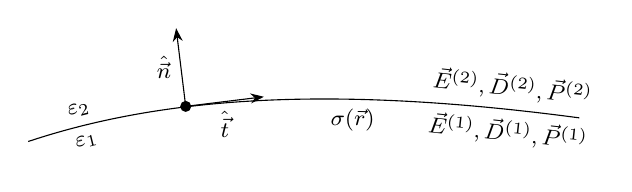
\begin{tikzpicture}[scale=1]
    \draw
    (0,0) .. controls (1.8,.6) and +(-3,.4) .. (7,.3)
    node[pos=.9, above, sloped] {$\vec E^{(2)},\vec D^{(2)},\vec P^{(2)}$}
    node[pos=.9, below, sloped] {$\vec E^{(1)},\vec D^{(1)},\vec P^{(1)}$}
    node[very near start, above, sloped] {$\varepsilon_2$}
    node[very near start, below, sloped] {$\varepsilon_1$}
    node[pos=.65,below,sloped] {$\sigma(\vec r)$};

    \coordinate (P) at (2, .446);

    \node[point] at (P) {};
    \draw[arr]
    (P) -- +(7:1)
    node[midway, below] {$\hat{\vec t}$};
    \draw[arr]
    (P) -- +(97:1)
    node[midway, left] {$\hat{\vec n}$};
    \end{tikzpicture}
}


\newcommand{\tfigDielektrischeBrechung}{
    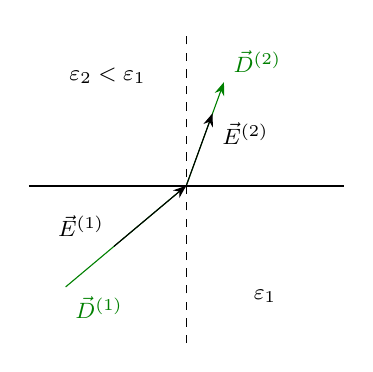
\begin{tikzpicture}[
        scale=2,
        incolor/.style = {red!50!black},
        outcolor/.style = {blue!50!black}
    ]
    \coordinate (Start) at (-140:1);
    \coordinate (StartFoot) at ($(Start) + (0,.2)$);
    \coordinate (Middle) at (0,0);
    \coordinate (End) at (70:0.7);
    \coordinate (EndFoot) at (0,0.2);

    \draw[arr,legreen] 
        (Start) -- (Middle) 
        node[at start,anchor=north west] {$\vec D^{(1)}$}
        (Middle) -- (End)
        node[at end,anchor=south west] {$\vec D^{(2)}$};
    \draw[arr] ($.6*(Start)$) -- (Middle) 
        node[at start,anchor=south east] {$\vec E^{(1)}$};
    \draw[arr] 
        (Middle) -- ($.7*(End)$)
        node[at end,anchor=north west] {$\vec E^{(2)}$};

    \draw[thick] (-1,0) -- +(2,0);
    \draw[dashed] (0,-1) -- +(0,2);
    \node at (-0.5,.7) {$\varepsilon_2<\varepsilon_1$};
    \node at (0.5,-.7) {$\varepsilon_1$};
    \end{tikzpicture}
}


\newcommand{\tfigMessungVonFeldDurchRandbedingungen}{
    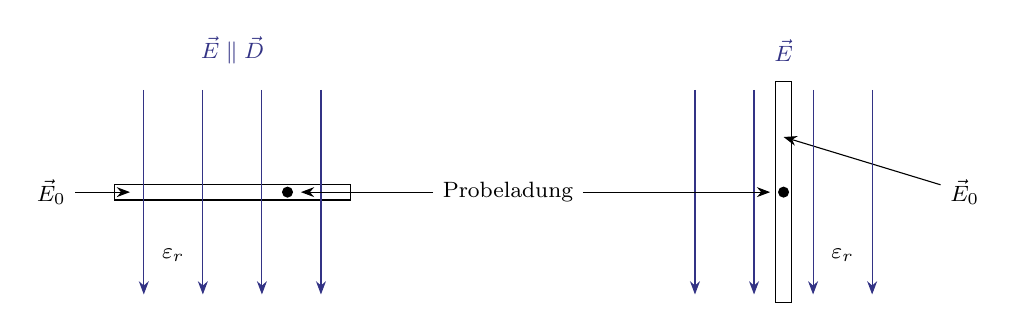
\begin{tikzpicture}[probeladung/.style={point,outer sep=1mm}]
    \draw[yshift=-1mm] (-5,0) rectangle +(3,.2);
    \node (E0) at (-5.8,0) {$\vec E_0$} edge[arr] (-4.8,0);
    \node[probeladung] (P1) at (-2.8,0) {};
    \node at (-5+3/4,-.8) {$\varepsilon_r$};
    \foreach \x in {1,2,...,4}{
        \draw[arr, object color] (3/4*\x-5-3/8,1.3) -- +(0,-2.6);
    };

    \draw[xshift=-1mm] (3.5,1.4) rectangle +(.2,-2.8);
    \node (E0) at (5.8,0) {$\vec E_0$} edge[arr] (3.5,0.7);
    \node[probeladung] (P2) at (3.5,0) {};
    \node at (5-3/4,-.8) {$\varepsilon_r$};
    \foreach \x in {1,2,...,4}{
        \draw[arr, object color] (3/4*\x+2-3/8,1.3) -- +(0,-2.6);
    };
    \node[object color] at (-3.5,1.8) {$\vec E\parallel\vec D$};
    \node[object color] at (3.5,1.8) {$\vec E$};

    \node at (0,0) {Probeladung} edge[arr] (P1) edge[arr] (P2);
    \end{tikzpicture}
}

\newcommand{\tfigDielektrischeKugelHomogenesEFeld}{
    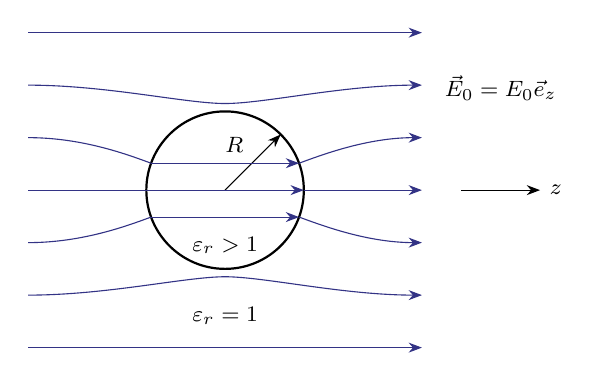
\begin{tikzpicture}[scale=1,earr/.style={arr,object color}]
    \draw[thick] (0,0) circle[radius=1];
    \draw[arr] (0,0) -- (45:1) node[midway, anchor=south east] {$R$};
    \node at (0,-.7) {$\varepsilon_r> 1$};
    \draw[earr] (-2.5,2) -- +(5,0);
    \draw[earr] (-2.5,-2) -- +(5,0);
    \draw[earr] (-2.5,0) -- (-1,0) (1,0) -- +(1.5,0);
    \foreach \i in {1,-1} {
        \draw[earr] (-2.5,\i*2/3) .. controls +(0:.7) and +(\i*160:.3) .. (\i*160:1) (\i*20:1) .. controls +(\i*20:.3) and +(\i*180:.7) .. (2.5,\i*2/3); 
        \draw[earr] (-2.5,\i*4/3) .. controls +(0:1) and +(180:.5) .. (0,\i*1.1) .. controls +(0:.5) and +(180:1) .. (2.5,\i*4/3);
    };

    \draw[earr] (160:1) -- (20:1);
    \draw[earr] (180:1) -- (0:1);
    \draw[earr] (-160:1) -- (-20:1);

    \draw[arr] (3,0) -- +(1,0) node[at end, right] {$z$};

    \node at (0,-1.6) {$\varepsilon_r=1$};
    \node at (3.5,1.3) {$\vec E_0=E_0\vec e_z$};
    \end{tikzpicture}
}

\newcommand{\tfigEntelektrisierung}{
    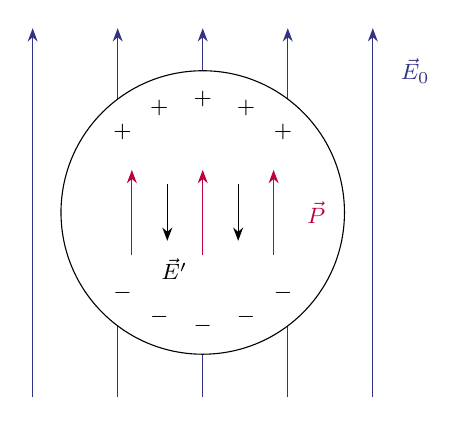
\begin{tikzpicture}[scale=1.8]
        \foreach \x in {0,1,...,4}
            \draw[arr, object color] (-1.2+2.4*\x/4, -1.3) -- +(0,2.6);
        \draw[fill=white] (0,0) circle[radius=1]; 
        \foreach \x in {0,1,...,4} {
            \node at (135 - \x*90/4:.8) {$+$};
            \node at (-45 - \x*90/4:.8) {$-$};
        };
        \foreach \i in {0,1,2}
            \draw[arr,polarisation color] (-.5+\i/2,-.3) -- +(0,.6);
        \foreach \i in {0,1}
            \draw[arr] (-.25+\i/2,.2) -- +(0,-.4);
        
        \node[object color] at (1.5,1) {$\vec E_0$};
        \node[polarisation color] at (.8,0) {$\vec P$};
        \node[] at (-.2,-.4) {$\vec E'$};
    \end{tikzpicture}
}


\newcommand{\tfigSimpleDielectricBodiesEntelektrisierungsfeld}{
    \begin{tikzpicture}
        \foreach \i in {0,...,5}{
            \foreach \y in {-1,0,1}{
                \draw[arr,object color] (\i*3-1,\y*.4) -- +(2,0);
            }
        }
        \draw[thick] (0,0) circle[radius=.7];
        \begin{scope}[xshift=3cm]
            \draw[thick,rotate=45] (0,0) ellipse[x radius=.7,y radius=.5];
        \end{scope}
        \draw[thick] (6-.1,-.8) -- +(0,1.6)(6+.1,-.8) -- +(0,1.6);
        \draw[thick] (9-.8,.2) -- +(1.6,0) (9-.8,-.2) -- +(1.6,0);
        
        \draw[thick] let \n1={12-.8},\n2={12+.7} in
        (\n1,.2) -- +(\n2-\n1,0) (\n1,-.2) -- +(\n2-\n1,0) 
        (\n1,0) ellipse[y radius=.2,x radius=.1]
        (\n2,.2) arc[y radius=.2,x radius=.1,start angle=90, end angle=-90];
        
        \draw[thick] let \n1={15-.2},\n2={15+.2} in
        (\n1,-.8) -- +(0,1.6) (\n2,-.8) -- +(0,1.6) 
        (15,.8) ellipse[x radius=.2,y radius=.1]
        (\n1,-.8) arc[x radius=.2,y radius=.1,start angle=-180, end angle=0];
        
        \node at (0,-1.5) {$\displaystyle\lambda=\frac13$};
        \node at (3,-1.5) {$\lambda=\begin{pmatrix}\lambda_1&0&0\\0&\lambda_2&0\\0&0&\lambda_3\end{pmatrix}$};
        \node at (6,-1.5) {$\lambda=1$};
        \node at (9,-1.5) {$\lambda=0$};
        \node at (12,-1.5) {$\lambda=0$};
        \node at (15,-1.5) {$\displaystyle\lambda=\frac12$};
    \end{tikzpicture}
}


\newcommand{\tfigClausiusMosotti}{
    % dipol in dielektrikum in äußerem Feld - Beschreibung durch lokale dipole
    \begin{tikzpicture}[scale=1]
        \draw[arr, object color] (-2,-2) -- +(0,4) node[anchor=south west] {$\vec E_0$};
        \draw (-2.3,-1.7) -- +(7.3,0) (-2.3,1.7) -- +(7.3,0);

        \draw[fill=white] (0,0) circle[radius=1]; 
        \foreach \x in {0,1,...,3} {
            \node at (135 - \x*90/3:1.2) {$-$};
            \node at (-45 - \x*90/3:1.2) {$+$};
        }; 
        
        \draw[arr,polarisation color] (0,-.3) -- +(0,.6) node[midway,right] {$\vec p$};
        \foreach \i in {0,1,...,4}
            \draw[arr] ($(12+\i*360/5:.7)+(0,-.2)$) -- +(0,.4);
        \draw[arr] (2.5,0) -- +(0,1) node[midway,right,xshift=2mm] {$\displaystyle\vec E=\frac{1}{\varepsilon_r}\vec E_0$};
        \node[polarisation color] at (1.5,0) {$\vec P$};
        \node at (3.5,-1) {$\varepsilon_r>1$};
    \end{tikzpicture}
}


\newcommand{\tfigMagnetfeldBeiLeiter}{
    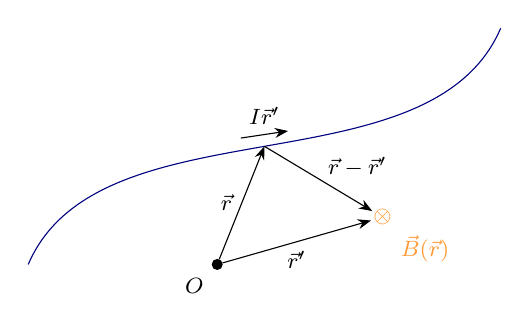
\begin{tikzpicture}[scale=3]
        \coordinate (O) at (0. 8,0);   % Koordinatenursprung
        \coordinate (A) at (1, 0.5);   % Punkt auf Leiter
        \coordinate (B) at (1.5, 0.2); % Punkt, wo Magnetfeld ausgewertet wird
        
        % Leiter (Kurve)
        \draw[color=blue!50!black] (0,0) .. controls (.3,.7) and (1.7,.3) .. (2,1);
        % Stromelement Idr
        \draw[arr] (1-0.1, 0.55-0.015) -- +(0.2, 0.03) 
            node[midway, above] {$I \diff \vec r'$}; 
            
        % Punkt, wo Magnetfeld ausgewertet wird
        \node[invisible point,text=orange!80] (b point) at (B) 
            [label={south east}:\textcolor{orange!80}{$\vec B(\vec r)$}] {$\mathbf{\otimes}$};
        % Punkt auf Leiter
        \node[invisible point] (conductor point) at (A) {}
            edge[arr] node[midway,auto,yshift=-1mm] {$\vec r-\vec r'$} 
            (b point);
        % Ursprung
        \node[point] (origin) at (O) [label={south west}:$O$] {} 
            edge[arr] node[midway,left] {$\vec r$} 
            (conductor point) 
            edge[arr] node[midway,below] {$\vec r'$} 
            (b point);
            
    \end{tikzpicture}
}

\newcommand{\tfigKraftParalleleLeiter}{
    \begin{tikzpicture}[scale=1.5,distance marker nobar/.style={<->,>={Stealth}},]
        \draw[distance marker nobar] (0,0.8) -- +(1,0) node[midway, above] {$d$};
        \draw[object color,midarrow] (0,-1) -- +(0,2) node[pos=.75,left] {$I_1$};
        \draw[object color,midarrow] (1,1) -- +(0,-2) node[pos=.25,right] {$I_2$};
        \draw[arr] (0,-.5) -- +(-.4,0) node[left] {$\diff\vec F$};
        \draw[arr] (1,-.5) -- +(.4,0);
        
        \begin{scope}[xshift=4cm]
            \draw[distance marker nobar] (0,0.8) -- +(1,0) node[midway, above] {$d$};
            \draw[object color,midarrow] (0,-1) -- +(0,2) node[pos=.75,left] {$I_1$};
            \draw[object color,midarrow] (1,-1) -- +(0,2) node[pos=.75,right] {$I_2$};
            \draw[arr] (0,-.5) -- +(.4,0) node[at start, left] {$\diff\vec F$};
            \draw[arr] (1,-.5) -- +(-.4,0);
        \end{scope}
    \end{tikzpicture}
}


\newcommand{\tfigCylinderConductorJandB}{
    \begin{tikzpicture}
        \draw[arr] (0,-1) -- +(0,4.5) node[anchor=south east] {$z$};
        
        \draw[arr] ($(100:.5)-(0,.7)$) arc[start angle=-260, end angle=80,x radius=.5, y radius=.25] node[pos=.75,right] {$\vec B$};
        
        \draw (-.7,2.5) -- ++(0,-2) arc [x radius=0.7, y radius=0.35, start angle=-180, end angle=0] -- ++(0,2) +(-.7,0) ellipse[x radius=0.7, y radius=0.35];
        \draw[arr] (-.2,1) -- +(0,.8) node[midway, left] {$\vec j$};
        \draw[arr] (0,1.4) -- +(1,0) node[midway, above] {$\vec r$};
        \draw[arr] (0,.5) -- +(.7,0) node[midway, above] {$R$};
        
        \begin{scope}[xshift=3cm]
            \coordinate (C) at (0,1.5);
            \draw[midarrow] (C) circle[radius=.7] circle[radius=1.2] node[pos=.5] {$C$};
            \draw[arr] (C) -- +(.7,0) node[midway, below] {$R$};
            \draw[arr] (C) -- +(40:1.2) node[near end, anchor=south east] {$r$};
            
        \end{scope}
        
        \begin{scope}[xshift=5.5cm]
            \coordinate (A) at (2, 1.7);
            
            \draw[arr] (0,0) -- (0, 3) 
                node[at end, anchor=south east] {$j(r)$};
            \draw[arr] (0,0) -- (4, 0) 
                node[at end, anchor=north west] {$r$};
            \draw[charge color] let \p1 = (A) in
                (0, \y1) -- (A) 
                node[at start, left] {$j_0$}
                -- (\x1, 0)
                node[charge color, below] {$R$};
        \end{scope}
            
        \begin{scope}[xshift=11cm]
            % electric field
            \draw[arr] (0,0) -- +(0, 3) 
                node[at end, anchor=south east] {$B(r)$};
            \draw[arr] (0,0) -- +(4, 0) 
                node[at end, anchor=north west] {$r$};
                
            \draw[charge color] 
                let \n0={2},\n1={1.7},\n3={3.7}, in
                plot[domain=0:\n0] (\x,\x) 
                node[above left] at (\n0/2,\n0/2) {$\propto r$} 
                plot[domain=\n0:\n3] (\x,\n0*\n0/\x)
                let \n5={\n0+(\n3-\n0)/2} in % x value of middle point of second graph 
                node[above] at (\n5,\n0*\n0/\n5) {$\displaystyle\propto\frac{1}{r}$};
            \draw[dashed, very thin]  let \n0={2} in (\n0,\n0) -- +(0,-\n0) node[below] {$R$};
        \end{scope}
    \end{tikzpicture}
}


\newcommand{\tfigCoil}{
    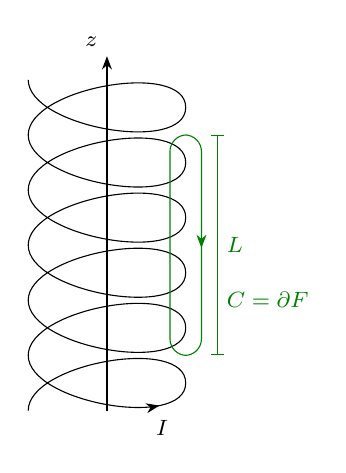
\begin{tikzpicture}[scale=1]
        \draw[arr] (0,0) -- (0,4.5)
        node[anchor=south east] {$z$};

        \draw[rmidarrow=.10] (-1,0)
        \foreach \a in {1,...,6}{
                .. controls +(0,.6) and +(0,.6)
                .. +(2,.35)
                .. controls +(0,-.6) and +(0,-.6)
                .. ++(0,.7)
            };
        \node[anchor=north west] at (.5,0) {$I$};
        \draw[legreen, rounded corners=6pt, midarrow=.7]
        (.8,.7) rectangle (1.2,3.5);
        \draw[legreen, |-|] (1.4,.7) -- +(0,2.8)
        node[midway, right] {$L$}
        node[near start, right] {$C=\partial F$};
    \end{tikzpicture}
}


\newcommand{\tfigMagnDipoleFieldCircleConductorEllipsoid}{
    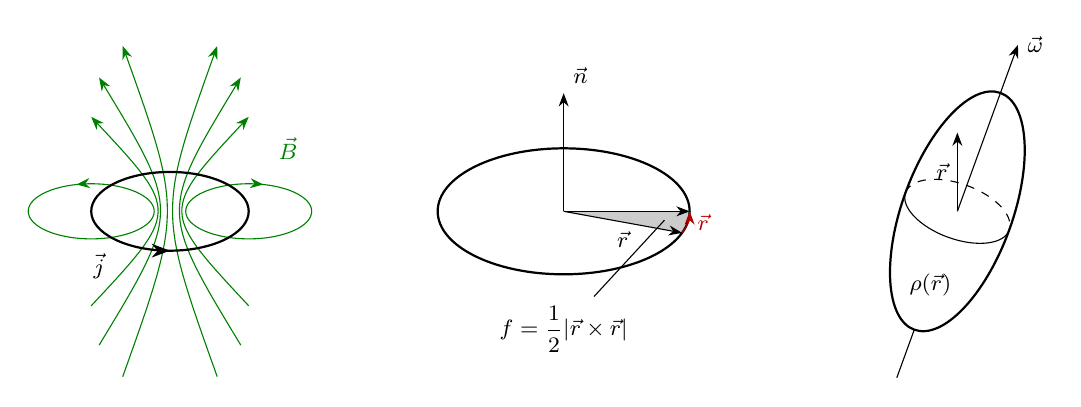
\begin{tikzpicture}
        \foreach \i in {-1,1}{
            \draw[legreen,arr] (-\i,-1.2) .. controls (\i*.12,0) .. +(0,2.4);
            \draw[legreen,arr] (-\i*.9,-1.7) .. controls (\i*.13,0) .. +(0,3.4);
            \draw[legreen,arr] (-\i*.6,-2.1) .. controls (\i*.15,0) .. +(0,4.2);
        }
        \draw[legreen,arr,midarrow=.3] (-1,0) ellipse[x radius=.8, y radius=.35];
        \draw[legreen,arr,rmidarrow=.2] (1,0) ellipse[x radius=.8, y radius=.35];
        
        \draw[midarrow=.75,thick] (0,0) ellipse[x radius=1, y radius=.5];
        \node at (-.9,-.7) {$\vec j$};
        \node[legreen] at (1.5,.8) {$\vec B$};
        
        \begin{scope}[xshift=5cm,xscale=2]
            \fill[black!20!white] (0,0) -- (.8,0) arc[radius=.8,start angle=0, end angle=-20] -- cycle;
            \draw[thick] (0,0) ellipse[x radius=.8, y radius=.8];
            \draw[arr] (0,0) -- (0,1.5) node[anchor=south west] {$\vec n$};
            \draw[arr] (0,0) -- (0:.8);
            \draw[arr] (0,0) -- (-20:.8) node[midway, below] {$\vec r$};
            \draw[arr, red laser] (-20:.8) arc[radius=.8,start angle=-20, end angle=0] node[midway, right] {$\diff\vec r$};
            
            \node at (0,-1.5) {$\displaystyle\diff f=\frac12|\vec r\times \diff\vec r|$} edge (-10:.65); 
        \end{scope}
        \begin{scope}[xshift=10cm]
            \begin{scope}[rotate=-20,yscale=.5]
                \draw[thick] (0,0) ellipse[x radius=.7, y radius=3.2];
                \draw (-.7,0) arc[x radius=.7, y radius=.7,start angle=-180, end angle=0];
                \draw[dashed] (-.7,0) arc[x radius=.7, y radius=.7,start angle=180, end angle=0];
                \node at (0,-2) {$\rho(\vec r)$};
                \draw[arr] (0,-4.5) -- (0,-3.2) (0,0) -- (0,4.5) node[right] {$\vec\omega$};
            \end{scope}
            \draw[arr] (0,0) -- (0,1) node[midway, left] {$\vec r$};
        \end{scope}
    \end{tikzpicture}
}

\newcommand{\tfighysterese}{
    \begin{tikzpicture}[scale=2]

        \coordinate (saturation) at (1,1);
        \coordinate (inv saturation) at (-1,-1);

        % Axis
        \draw[name path=xaxis,arr] (-1.4,0) -- (1.4,0) node[anchor=north west] {$H$};
        \draw[name path=yaxis,arr] (0,-1.4) -- (0,1.4) node[anchor=south east] {$B$};

        % Curve (1) (magnetize)
        \draw[midarrow,dashed,color=blue!50!black]
        (0,0) .. controls (0.3,.2) and (0.1,1) .. (saturation)
        node[midway,right,xshift=-1.5mm,yshift=-2mm] {(1)};
        % Curve (2)  (change field to negative)
        \draw[name path=dcurve, midarrow,color=blue!50!green]
        (saturation) .. controls (-0.8,1) and (-0.1,-1) .. (inv saturation)
        node[near end,left] {(2)};
        % Curve (2)  (change field to positive)
        \draw[midarrow,color=blue!60!white!70!black]
        (inv saturation) .. controls (0.8,-1) and (0.1,1) .. (saturation)
        node[near start,right,xshift=1mm,yshift=1mm] {(3)};
        % Coordinates of Saturation
        \draw[dashed] (saturation) -- (1,0)
        node[below] {$H_\mathrm{S}$};
        \draw[dashed] (saturation) -- (0,1)
        node[left] {$B_\mathrm{S}$};

        % Remanence and coercitive field
        \path[name intersections={of=yaxis and dcurve, by=remanenz}];
        \path[name intersections={of=xaxis and dcurve, by=coercitive}];
        \draw ($(remanenz)+(1pt,0)$) -- ($(remanenz)-(1pt,0)$)
        node[left] {$B_\mathrm{R}$};
        \draw ($(coercitive)+(0,1pt)$) -- ($(coercitive)-(0,1pt)$)
        node[anchor=north west,xshift=-2mm] {$H_\mathrm{C}$};

    \end{tikzpicture}
}

\newcommand{\tfigMagneticRefraction}{
    \begin{tikzpicture}[
            scale=2,
            incolor/.style = {red!50!black},
            outcolor/.style = {blue!50!black}
        ]
        \coordinate (Start) at (-2,-0.5);
        \coordinate (StartFoot) at ($(Start) + (0,.2)$);
        \coordinate (Middle) at (0,-0.3);
        \coordinate (End) at (0.4,0.2);
        \coordinate (EndFoot) at (0,0.2);

        \draw (0,1) -- (0,-.6);
        \node[circle] at (-1,.9) {$\mu_1$};
        \node[circle] at (.5,.9) {$\mu_2\gg\mu_1$};

        \draw[arr, incolor] (Start) -- (Middle)
        node[midway, below] {$\vec H^{(1)}$};
        \draw[arr, outcolor] (Middle) -- (End)
        node[midway, right] {$\vec H^{(2)}$};
        \draw[dashed, incolor] (Start) -- (StartFoot)
        node[midway,left] {$H_\parallel^{(1)}$}
        -- (Middle) node[midway, above] {$H_\perp^{(1)}$};
        \draw[dashed, outcolor] (EndFoot)
        -- (End) node[midway, above] {$H_\perp^{(2)}$};
    \end{tikzpicture}
}


\newcommand{\tfigConductorLoopWithRefPoint}{
    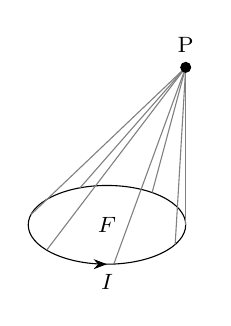
\begin{tikzpicture}[scale=1]
        \coordinate (O) at (0,0);
        \coordinate (P) at (1,2);
        \draw[midarrow=.75] (O) ellipse [x radius=1, y radius=.5]
        node[] {$F$};
        \node[below] at (0,-.5) {$I$};
        \foreach \angle in{0, 55, ..., 360}
        \draw[gray] ($cos(\angle)*(1,0)+sin(\angle)*(0,.5)$) -- (P);
        \node[point] at (P) [label=P]{};
    \end{tikzpicture}
}

% \newcommand{\tfigMagneticFeldHomogenousBall}{
%     \begin{tikzpicture}[
%             scale=.7,
%             mcolor/.style=legreen,
%             pics/graph/.style={background code={
%                             \coordinate (O) at (0,0);
%                             \coordinate (P) at (1,2);
%                             \draw (O) circle [radius=1];
%                             \foreach \vzx in {1,-1}{
%                                     \draw[midarrow] (\vzx*0.5,0.866) ..
%                                     controls ($1.2*(\vzx*0.5,0.866)$)
%                                     and (\vzx*1.2, 2.4) .. (\vzx*2.5,3);
%                                     \draw[midarrow] (\vzx*2.5,-3) ..
%                                     controls (\vzx*1.2,-2.4)
%                                     and ($1.2*(\vzx*0.5,-0.866)$) .. (\vzx*0.5,-0.866);
%                                     \draw[midarrow=.51] (\vzx*0.866,0.5)
%                                     .. controls +($.8*(\vzx*0.866,0.5)$)
%                                     and (\vzx*3,1)
%                                     .. (\vzx*3,0)
%                                     .. controls (\vzx*3,-1) and ($1.6*(\vzx*0.866,-0.5)$)
%                                     .. (\vzx*0.866,-0.5) ;
%                                     \draw[arr] (\vzx*0.866,#1*-0.4) -- (\vzx*0.866,#1*0.4);
%                                     \draw[arr] (\vzx*0.5,#1*-0.8) -- (\vzx*0.5,#1*0.8);
%                                     \draw[arr, mcolor] (\vzx*0.7,-0.4) -- +(0,0.8);
%                                     \draw[arr, mcolor] (\vzx*0.25,-0.4) -- +(0,0.8);
%                                 }
%                             \draw[midarrow=.6] (0,1) -- (0,3.2);
%                             \draw[midarrow=.4] (0,-3.2) -- (0,-1);
%                             \draw[arr] (0,#1*-.9) -- (0,#1*0.9);
%                         }}
%         ]

%         %\pic=1 at (0,0) [transform shape]{graph};
%         %\pic at (7,0) [transform shape]{graph};

%         \draw (0,0) pic[transform shape] {graph=1} node[outer sep=70,above] {$\vec B$-Feld};
%         \draw (7,0) pic[transform shape] {graph=-1} node[outer sep=70,above] {$\vec H$-Feld};
%         \node[mcolor] at (-1.5,0) {$\vec M$};
%         \node[mcolor] at (-1.5+7,0) {$\vec M$};

%     \end{tikzpicture}
% }


\newcommand{\tfigInductionA}{
    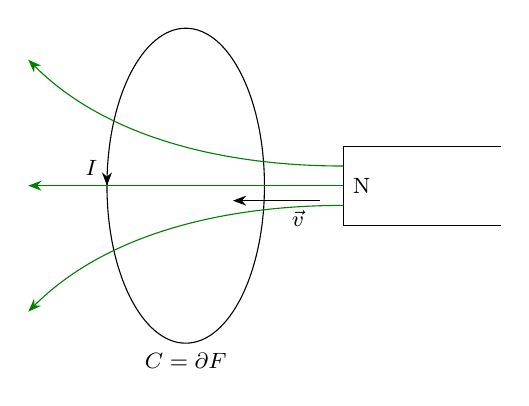
\begin{tikzpicture}[scale=1]
        \draw[midarrow=.5] (0,0)
        ellipse[x radius=1, y radius=2];

        \draw (4, -.5) -- ++(-2,0)
        -- ++(0,1) node[midway, right] {N}
        -- +(2,0);
        \draw[arr] (1.7,-.19) -- ++(-1.1,0) node[near start, below] {$\vec v$};
        \node[below] at (0,-2) {$C=\partial F$};
        \node[anchor=south east] at (-1,0) {$I$};
        \draw[legreen,arr] (2,0.25) .. controls +(-1.5,0) and +(1,-1) .. (-2,1.6);
        \draw[legreen,arr] (2,-0.25) .. controls +(-1.5,0) and +(1,1) .. (-2,-1.6);
        \draw[legreen,arr] (2,0) -- (-2,0);
    \end{tikzpicture}
}

\newcommand{\tfigInductionB}{
    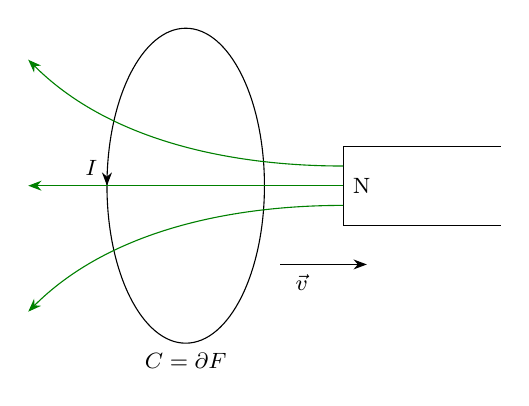
\begin{tikzpicture}[scale=1]
        \draw[midarrow=.5] (0,0)
        ellipse[x radius=1, y radius=2];

        \draw (4, -.5) -- ++(-2,0)
        -- ++(0,1) node[midway, right] {N}
        -- +(2,0);
        \draw[arr] (1.2,-1) -- ++(1.1,0) node[near start, below] {$\vec v$};
        \node[below] at (0,-2) {$C=\partial F$};
        \node[anchor=south east] at (-1,0) {$I$};
        \draw[legreen,arr] (2,0.25) .. controls +(-1.5,0) and +(1,-1) .. (-2,1.6);
        \draw[legreen,arr] (2,-0.25) .. controls +(-1.5,0) and +(1,1) .. (-2,-1.6);
        \draw[legreen,arr] (2,0) -- (-2,0);
    \end{tikzpicture}
}


\newcommand{\tfigcylindricalConductorAndCoil}{
    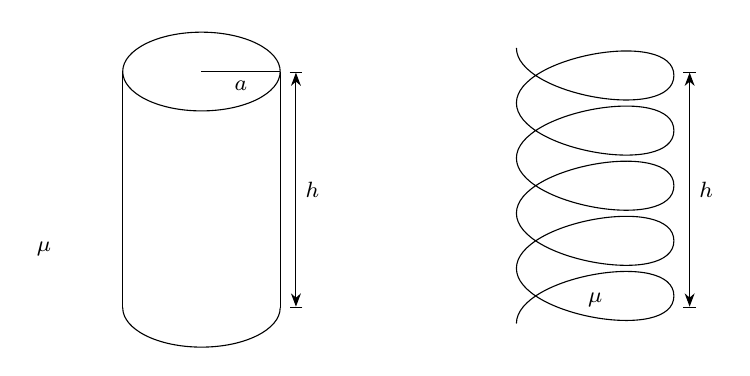
\begin{tikzpicture}[scale=1]
        \coordinate (bottom) at (0,0);
        \coordinate (top) at (0,3);
        \coordinate (offset) at (1,0);

        % cylindrical conductor
        \draw (top)
        ellipse[x radius=1, y radius=.5];
        \draw
        ($(bottom) + (offset)$)
        arc[start angle=0, end angle=-180, x radius=1, y radius=.5];
        \draw
        ($(bottom) + (offset)$) -- ($(top) + (offset)$)
        ($(bottom) - (offset)$) -- ($(top) - (offset)$);
        \draw
        (top) -- ($(top) + (offset)$)
        node[midway, below] {$a$};
        \draw[distance marker]
        ($(bottom) + (offset) + (.2, 0)$) -- +(top)
        node[midway, right] {$h$};
        \node at ($(bottom) + (-2,.75)$) {$\mu$};
        % coil
        \begin{scope}[shift={(4,0)}]
            \draw (0,-.2)
            \foreach \a in {1,...,5}{
                .. controls +(0,.6) and +(0,.6)
                .. +(2,.35)
                .. controls +(0,-.6) and +(0,-.6)
                .. ++(0,.7)
            };
            \node at (1,0.1) {$\mu$};
            \draw[distance marker]
                (2.2, 0) -- +(0,3)
                node[midway, right] {$h$};
        \end{scope}
    \end{tikzpicture}
}


\newcommand{\tfigTwoInductors}{
    \begin{tikzpicture}[scale=1]
        \draw[rotate=20, midarrow=0.75]
        (0,0) ellipse [x radius=1, y radius=.5]
        node {$C_1$}
        node[xshift=13, yshift=-20] {$I_1$};
        \draw[rotate=-40, midarrow=0.75]
        (3,0) ellipse [x radius=1, y radius=.5]
        node {$C_2$}
        node[xshift=-13, yshift=-20] {$I_2$};
        \node at (0,-2) {$\mu$};
        \node at (3,0) {$\ldots$};
    \end{tikzpicture}
}

\newcommand{\tfigGrenzflaecheMagnetic}{
    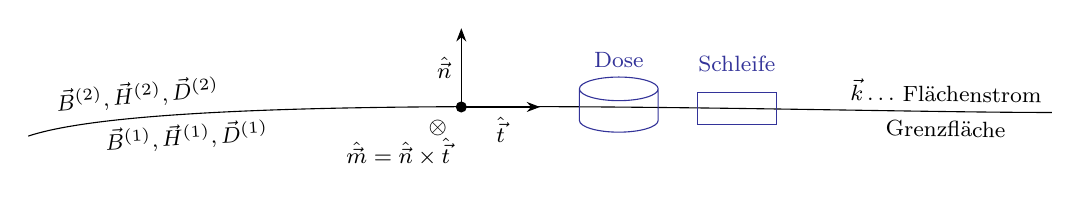
\begin{tikzpicture}[
            scale=1,
            dosenfarbe/.style={blue!50!black!80!white}
        ]
        \draw
        (0,0) .. controls (1.8,.6) and +(-3,0) .. (13,.3)
        node[pos=.17, above, sloped] {$\vec B^{(2)},\vec H^{(2)},\vec D^{(2)}$}
        node[pos=.22, below, sloped] {$\vec B^{(1)},\vec H^{(1)},\vec D^{(1)}$}
        node[very near end, above, sloped] {$\vec k\ldots$ Flächenstrom}
        node[very near end, below, sloped] {Grenzfläche};

        \coordinate (P) at (5.5, .37);

        \node[point] at (P) {};
        \draw[arr]
        (P) -- +(0:1)
        node[midway, below] {$\hat{\vec t}$};
        \draw[arr]
        (P) -- +(90:1)
        node[midway, left] {$\hat{\vec n}$};

        \node at (5.2,.1) {$\otimes$}
        node at(4.7,-.2) {$\hat{\vec m}=\hat{\vec n}\times\hat{\vec t}$};

        \draw [dosenfarbe]
        (7,.6) -- +(0,-.4)
        arc[start angle=-180, end angle=0,x radius=.5, y radius=.15]
        -- +(0,.4)
        arc[start angle=0, end angle=180,x radius=.5, y radius=.15]
        node[midway, above] {Dose}
        arc[start angle=-180, end angle=0,x radius=.5, y radius=.15];
        \draw[dosenfarbe]
        (8.5,.55) rectangle +(1,-0.4) node[midway,above,yshift=10] {Schleife};
    \end{tikzpicture}
}


\newcommand{\tfigBewegungDurchLichtaetherA}{
    \begin{tikzpicture}[scale=3]
        \begin{scope}
            \draw[arr] (0,0) -- (0,1)
                node[anchor=south east] {$\vec e_2$};
            \draw[arr] (0,0) -- (1,0)
                node[anchor=north west] {$\vec e_1$};
            \node at (.5,.5) {Äther};
        \end{scope}
        \begin{scope}[shift={(2cm,0)}]
            \draw[arr] (0,0) -- (0,1)
                node[anchor=south east] {$\vec e_2$};
            \draw[arr] (0,0) -- (1,0)
                node[anchor=north west] {$\vec e_1$};
            \node at (.5,.5) {Erde};

            \draw[arr] (.2,.2) -- +(.6,0) node[anchor=west] {$\vec v=v \vec e_1$};            
        \end{scope}
    \end{tikzpicture}
}

\newcommand{\tfigBewegungDurchLichtaetherB}{
    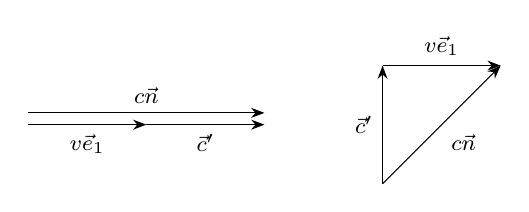
\begin{tikzpicture}[scale=1.5]
        \begin{scope}
            \draw[arr] (0,0) -- +(1,0)
                node[midway, below] {$v\vec e_1$};
            \draw[arr] (1,0) -- +(1,0)
                node[midway, below] {$\vec c'$};
            \draw[arr] (0,.1) -- +(2,0)
                node[midway, above] {$c \vec n$};
        \end{scope}

        \begin{scope}[shift={(3cm,-0.5cm)}]
            \draw[arr] (0,0) -- (0,1)
                node[midway, left] {$\vec c'$};
            \draw[arr] (0,1) -- +(1,0)
                node[midway, above] {$v\vec e_1$};
            \draw[arr] (0,0) -- +(1,1)
                node[midway, anchor=north west] {$c\vec n$};

        \end{scope}
    \end{tikzpicture}
}

\newcommand{\tfigMichelsonInterferometer}{
    \begin{tikzpicture}[scale=2]
        \coordinate (ST) at (0,0);
        \coordinate (L) at (-1,0);
        \coordinate (S1) at (0,1);
        \coordinate (S2) at (1,0);
        \coordinate (D) at (0,-1);

        \draw[midarrow, red laser] (L) -- (ST);
        \draw[midarrow=.3, rmidarrow=.6, red laser] (ST) -- (S1);
        \draw[midarrow=.3, rmidarrow=.6, red laser] (ST) -- (S2);
        \draw[midarrow, red laser] (ST) -- (D);

        \draw[dashed, very thick] ($(ST) + (45:.3)$) -- ($(ST) - (45:.3)$);
        \draw[very thick] ($(S1) + (.3,0)$) -- ($(S1) - (.3,0)$)
            node[midway, above] {S1};
        \draw[very thick] ($(S2) + (0,.3)$) -- ($(S2) - (0,.3)$)
            node[midway, right] {S2};
        
        \draw[fill=black] ($(L) - (.4, .1)$) rectangle ($(L) + (0, .1)$);
        \draw[fill=black] ($(D) - (.3, .05)$) rectangle ($(D) + (.3, 0)$)
            node[midway, below, yshift=-1.2mm] {D};

        \draw[|-|] let \p1 = (S1), \p2 = (S2) in 
            (\x2 + .4cm,\y1) -- (\x2 +.4cm, 0) 
            node[midway, right] {$l_1$};
        \draw[|-|] let \p1 = (S1), \p2 = (S2) in 
            (0,\y1 +.4cm) -- (\x2,\y1 +.4cm) 
            node[midway, above] {$l_2$};

        \begin{scope}[shift={(-2cm, -1cm)}, scale=.5]
            \draw[arr] (0,0) -- (0,1) node[anchor=south east] {$\vec e_2$};
            \draw[arr] (0,0) -- (1,0) node[anchor=north west] {$\vec e_1$};
        \end{scope}
    \end{tikzpicture}
}


\newcommand{\tfigSRTGedankenExperimentLichtkegel}{
    \begin{tikzpicture}[scale=2.5]

        \coordinate (O) at (0,0);
        \coordinate (O2) at (2.5,0.3);
        
        \draw[arr] (0,0) -- (0,1) node[anchor=south west] {$z$} node[midway, left] {$\Sigma$};
        \draw[arr] (0,0) -- (1,0) node[anchor=south west] {$x$};
        \draw[arr] (0,0) -- (45:0.8) node[anchor=north west] {$y$};

        \foreach \angle in {0,45,...,360}{
            \draw[arr, red laser] (O) -- (\angle:0.3);
        }
        \draw[arr] ($.7*(O2)$) -- ($0.9*(O2)$) node[midway, above] {$\vec v$};

        \begin{scope}[shift={(O2)}, moving system color]
            \draw[arr] (0,0) -- (0,1) node[anchor=south west] {$z'$} node[midway, left] {$\Sigma'$};
            \draw[arr] (0,0) -- (1,0) node[anchor=south west] {$x'$};
            \draw[arr] (0,0) -- (45:0.8) node[anchor=north west] {$y'$};
        \end{scope}
    \end{tikzpicture}
}
\renewcommand{\tfigSRTGedankenExperimentLichtkegel}{
    \begin{tikzpicture}[scale=3]
        \begin{scope}          
            \draw[arr] (0,0) -- (0,1) node[anchor=south west] {$y,\textcolor{blue!60!black!70!white}{y'}$} 
            node[midway, left] {$\Sigma,\textcolor{blue!60!black!70!white}{\Sigma'}$};
            \draw[arr] (0,0) -- (1,0) node[anchor=north west] {$x,\textcolor{blue!60!black!70!white}{x'}$};
            \node at (.5,-.2) {$t_0=0$};
        \end{scope}
        \begin{scope}[xshift=2cm]
            \node at (.5,-.2) {$t_0+\diff t$};

            \coordinate (O) at (0,0);
            \coordinate (O2) at (0.6,0.2);
            \coordinate (L) at (.9,.8);

            \draw[arr, red laser] (O) -- (L);
            \draw[arr, red laser] (O2) -- (L);

            \draw[gray,decorate, decoration = {brace}] let \p1 = (L) in 
                (0,\y1) -- (\x1,\y1) node[midway, above] {$\diff x$};
            \draw[gray,decorate, decoration = {brace}] let \p1 = (L) in 
                (\x1,0) -- (\x1,\y1) node[midway, left] {$\diff y$};
            
            \draw[arr] (0,0) -- (0,1) node[anchor=south west] {$y$} node[midway, left] {$\Sigma$};
            \draw[arr] (0,0) -- (1,0) node[anchor=north west] {$x$};
            %\draw[arr] (0,0) -- (45:0.8) node[anchor=north west] {$y$};

            \draw[arr] (O) -- (O2) node[midway, above] {$\vec v$};

            \begin{scope}[shift={(O2)}, moving system color]
                \draw[arr] (0,0) -- (0,1) node[anchor=south west] {$y'$} node[midway, left] {$\Sigma'$};
                \draw[arr] (0,0) -- (1,0) node[anchor=north west] {$x'$};
                %\draw[arr] (0,0) -- (45:0.8) node[anchor=north west] {$y'$};
                \draw[blue!50!gray,decorate,decoration = {brace}] let \p1 = (L) in 
                    (0,\y1+1) -- +(\x1,0) node[midway, above] {$\diff x'$};
                \draw[blue!50!gray,decorate, decoration = {brace,mirror}] let \p1 = (L) in 
                    (\x1+1,0) -- +(0,\y1) node[midway, right] {$\diff y'$};
            \end{scope}
        \end{scope}
    \end{tikzpicture}
}

\newcommand{\tfigSRTLichtkegel}{
    \begin{tikzpicture}[scale=2.5]
        \draw[arr] (0,-1) -- (0,1) node[anchor=south west] {$ct$};
        \draw[arr] (-1,0) -- (1,0) node[anchor=north west] {$x$};

        \draw[color=blue!50!green] (-.9,.9) -- (.9,-.9) (-.9,-.9) -- (.9,.9) 
        node[right] {$-(ct)^2+x^2=0$};
    \end{tikzpicture}
}



\newcommand{\tfigGeschwindigkeitsaddition}{
    \begin{tikzpicture}[scale=2]
        \begin{scope}
            \draw[arr] (0,0) -- (0,1)
                node[midway, left] {$\Sigma$}
                node[anchor=south east] {$y$};
            \draw[arr] (0,0) -- (1,0)
                node[anchor=north west] {$x$};
        \end{scope}
        \begin{scope}[shift={(2cm,0)}]
            \draw[arr] (0,0) -- (0,1)
                node[midway, left] {$\Sigma'$}
                node[anchor=south east] {$y'$};
            \draw[arr] (0,0) -- (1,0)
                node[anchor=north west] {$x'$};

            \draw[arr] (.2,.2) -- +(.6,0) node[anchor=west] {$v$};
            \node (U) at (.9,.6) {$u$};
            \node[point] at (.4,.6) {} edge[arr] (U);
        \end{scope}
    \end{tikzpicture}
}

\newcommand{\tfigMinkowskiDiagramA}{
    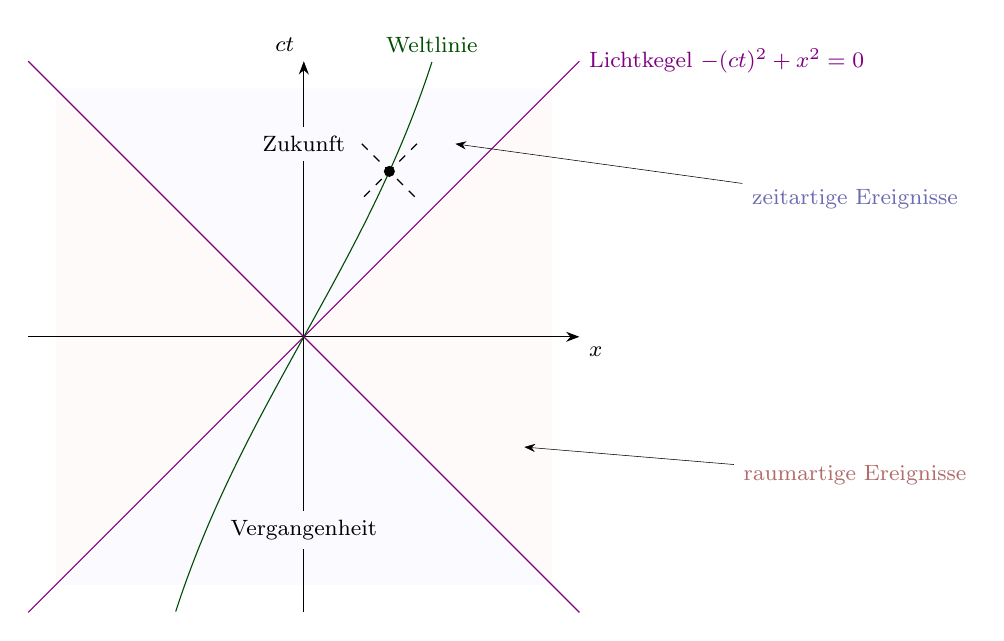
\begin{tikzpicture}[scale=3.5]
        \coordinate (C1) at (.9,.9);
        \coordinate (C2) at (-.9,.9);
        \coordinate (C3) at (-.9,-.9);
        \coordinate (C4) at (.9,-.9);

        \fill[blue!2!white] (C2) -- (C4) -- (C3) -- (C1);
        \fill[red!2!white] (C2) -- (C4) -- (C1) -- (C3);

        \draw[arr] (-1,0) -- (1,0) node[anchor=north west] {$x$};
        \draw[arr] (0,-1) -- (0,1) node[anchor=south east] {$ct$};
        \draw[color=violet] (-1,1) -- (1,-1) (-1,-1) -- (1,1) 
            node[right] {Lichtkegel $-(ct)^2+x^2=0$};
        
        \node[fill=blue!2!white] at (0,.7) {Zukunft};
        \node[fill=blue!2!white] at (0,-.7) {Vergangenheit};
        \node[red!40!white!70!black] at (2,-.5) {raumartige Ereignisse} edge[arr, very thin] (.8,-.4);
        \node[blue!40!white!70!black] at (2,.5) {zeitartige Ereignisse} edge[arr, very thin] (.55,.7);
        
        \draw[color=green!30!black, name path={weltlinie}] (-115:1.1) .. controls +(72:.8) and +(-108:.8) ..  (65:1.1)
            node[anchor=south] {Weltlinie};
        \draw[transparent, name path={x parallel}] (0,.6) -- +(.5,0);
        \draw[name intersections={of=weltlinie and x parallel,by={P1}},dashed] 
            ($(P1)+(.1,.1)$) -- ($(P1)+(-.1,-.1)$) 
            ($(P1)+(-.1,.1)$) -- ($(P1)+(.1,-.1)$)
            node[point] at (P1) {};
    \end{tikzpicture}
}
\newcommand{\tfigMinkowskiDiagramB}{
    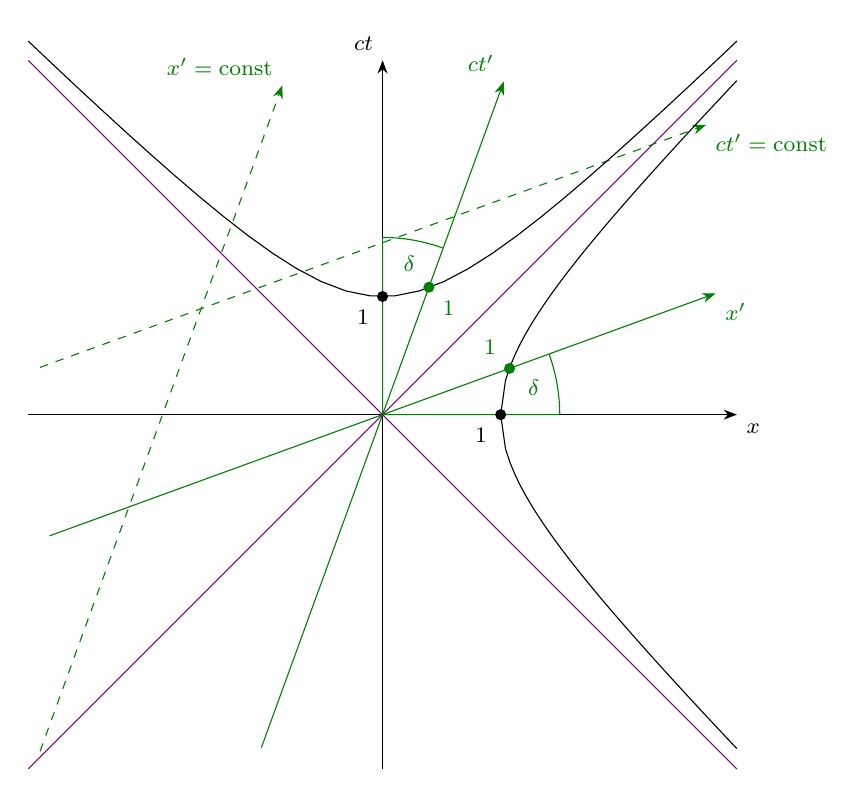
\begin{tikzpicture}[scale=1.5,clr/.style={legreen}]
        \draw[arr] (-3,0) -- (3,0) node[anchor=north west] {$x$};
        \draw[arr] (0,-3) -- (0,3) node[anchor=south east] {$ct$};
        \draw[color=violet] let \n1={3} in (-\n1,\n1) -- (\n1,-\n1) (-\n1,-\n1) -- (\n1,\n1);
    
        \draw[clr,arr,name path global/.expanded={ctp axis}] (-110:3) -- (70:3) node[anchor=south east] {$ct'$};
        \draw[clr,arr,name path global/.expanded={xp axis}] (-160:3) -- (20:3) node[anchor=north west] {$x'$};
        \draw[clr,arr,dashed] (-2.9,.4) -- +(20:6) node[anchor=north west] {$ct'=\mathrm{const}$};
        \draw[clr,arr,dashed] (-2.9,-2.85) -- +(70:6) node[anchor=south east] {$x'=\mathrm{const}$};
        
        \draw[name path global/.expanded={hyp top}] plot[domain=-3:3,samples=30] ({\x},{sqrt(1+\x*\x)});
        \draw[name path global/.expanded={hyp right}] plot[domain=1:3,samples=50] ({\x},{sqrt(\x*\x-1)});
        \draw plot[domain=1:3,samples=50] ({\x},{-sqrt(\x*\x-1)});
        
        \draw[clr] (0,0) -- (1.5,0) arc [start angle=0, end angle=20, radius=1.5];
        \draw (10:1.3) node[clr] {$\delta$};
        \draw[clr] (0,0) -- (0,1.5) arc [start angle=90, end angle=70, radius=1.5];
        \draw (80:1.3) node[clr] {$\delta$};
    
        \node[point] at (1,0) [label={south west}:1] {};
        \node[point] at (0,1) [label={south west}:1] {};
        
        \path [name intersections={of=ctp axis and hyp top,by={P1}}]
            (P1) node [point,clr,label={south east,clr}:1] {};
        \path [name intersections={of=xp axis and hyp right,by={P1}}]
            (P1) node [point,clr,label={north west,clr}:1] {};
    \end{tikzpicture}
}



\newcommand{\tfigMinkowskiZeitdilatationLaengenkontraktion}{
    % Zeitdilatation und Längenkontraktion
    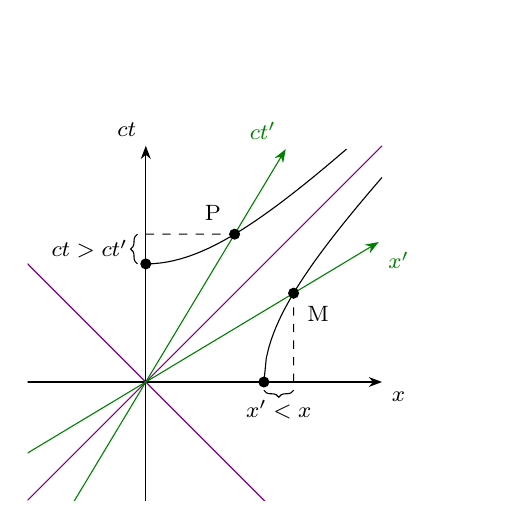
\begin{tikzpicture}[scale=1.5,clr/.style={legreen}]
        \clip (-1,-1) rectangle (3,3);
        \draw[arr] (-2,0) -- (2,0) node[anchor=north west] {$x$};
        \draw[arr] (0,-2) -- (0,2) node[anchor=south east] {$ct$};
        \draw[color=violet] let \n1={2} in (-\n1,\n1) -- (\n1,-\n1) (-\n1,-\n1) -- (\n1,\n1);
        \path let \n1={31},\n2={2.3} in 
            coordinate (A) at (-90-\n1:\n2)
            coordinate (B) at (90-\n1:\n2)
            coordinate (C) at (-180+\n1:\n2)
            coordinate (D) at (\n1:\n2);
        
        \draw[clr,arr,name path global/.expanded={ctp axis}] (A) -- (B) node[anchor=south east] {$ct'$};
        \draw[clr,arr,name path global/.expanded={xp axis}] (C) -- (D) node[anchor=north west] {$x'$};
        \draw[name path global/.expanded={hyp top}] plot[domain=0:1.7,samples=30] ({\x},{sqrt(1+\x*\x)});
        \draw[name path global/.expanded={hyp right}] plot[domain=1:2,samples=50] ({\x},{sqrt(\x*\x-1)});

        \node[point] at (1,0) {};
        \node[point] at (0,1) {};
        
        \path [name intersections={of=ctp axis and hyp top,by={P1}}]
            (P1) node [point,label={north west}:P] {};
        \path [name intersections={of=xp axis and hyp right,by={P2}}]
            (P2) node [point,label={south east}:M] {};
        \draw[dashed] let \p1=(P1),\p2=(P2) in 
            coordinate (PCT) at (0,\y1) 
            coordinate (PX) at (\x2,0) 
            (PCT) -- (P1)
            (PX) -- (P2);
        
        \draw[decorate, decoration = {brace,raise=3pt}] 
        (0,1) -- (PCT) node[midway, left,xshift=-3pt] {$ct>ct'$};
        \draw[decorate, decoration = {brace,raise=3pt}] 
        (PX) -- (1,0) node[midway, below,yshift=-3pt] {$x'<x$};
    \end{tikzpicture}
}


\newcommand{\tfigZunahmeImpulsmasse}{
    \begin{tikzpicture}
        \draw[arr] (0,0) -- (0,3) node[anchor=south east] {$m_r=\gamma m$}; 
        \draw[arr] (0,0) -- (3,0) node[anchor=north west] {$v/c$};
        \draw (-.1,1) -- +(.2,0) node[at start, left] {$m$};
        % hack: we parametrize with sqrt(x) so the precision goes up for values near 1:
        \draw plot[domain=0:.88,smooth] ({sqrt(\x)*2},{1/sqrt(1-\x)}); 
        \draw[dashed] (2,-.1) -- +(0,3) node[at start, below] {1};
    \end{tikzpicture}
}


\newcommand{\tfigMassenschale}{
    \begin{tikzpicture}
        \draw[arr] (0,-1) -- (0,3) node[anchor=south east] {$p^0$}; 
        \draw[arr] (-2.5,0) -- (2.5,0) node[anchor=north west] {$\vec p$};
        \draw[dashed] let \n1={2} in (-2,2) -- (1,-1) (2,2) -- (-1,-1);
        \draw plot[domain=-2:2] (\x,{sqrt(\x*\x+1)});
        \draw (-.1,1) -- +(.2,0) node[at start, anchor=north east] {$mc$};
    \end{tikzpicture}
}